\documentclass[border=1pt]{standalone}
\usepackage{amsmath,amssymb}
\usepackage{pgfplots}
\pgfplotsset{compat=1.18}
\usepgfplotslibrary{groupplots}
\usepackage{pgfplotstable}
\setlength{\textwidth}{5.0in}
\setlength{\linewidth}{5.0in}
\begin{document}
\pgfplotstableread[col sep=comma]{figdata/regime_compacton.csv}\regimeA
\pgfplotstableread[col sep=comma]{figdata/regime_solitary.csv}\regimeB
\pgfplotstableread[col sep=comma]{figdata/regime_algebraic.csv}\regimeC
\pgfplotstableread[col sep=comma]{figdata/regime_cnoidal.csv}\regimeD
\pgfplotstableread[col sep=comma]{figdata/profile_compacton.csv}\compactondata
\pgfplotstableread[col sep=comma]{figdata/profile_a0.01.csv}\profileAA
\pgfplotstableread[col sep=comma]{figdata/profile_a0.10.csv}\profileAB
\pgfplotstableread[col sep=comma]{figdata/profile_a0.50.csv}\profileAC
\pgfplotstableread[col sep=comma]{figdata/profile_a1.00.csv}\profileAD
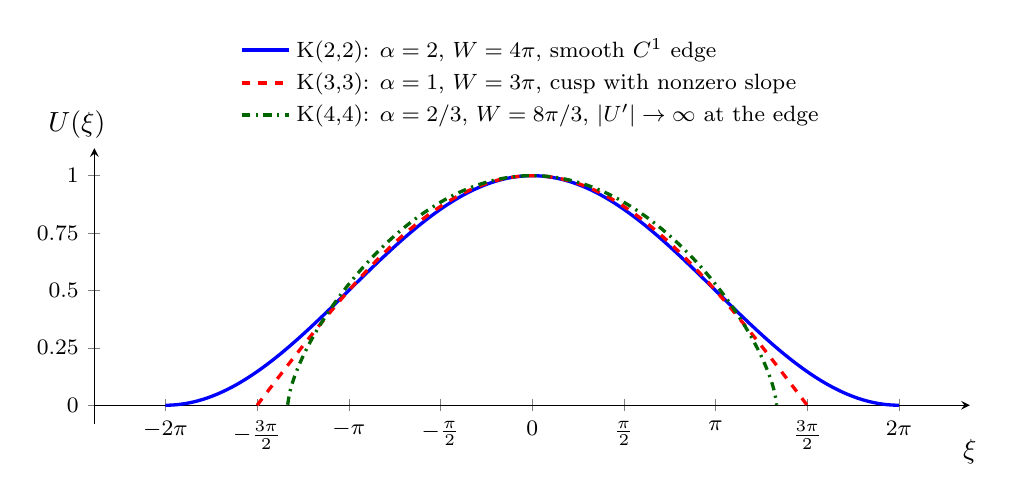
\begin{tikzpicture}
\begin{axis}[
    width=\textwidth,
    height=0.40\textwidth,
    xlabel={$\xi$},
    ylabel={$U(\xi)$},
    xmin=-7.5, xmax=7.5,
    ymin=-0.08, ymax=1.12,
    legend columns=1,
    legend cell align=left,
    legend style={
      at={(0.5,1.04)},
      anchor=south,
      font=\footnotesize,
      draw=none,
    },
    axis x line=middle,
    axis y line=left,
    every axis x label/.style={at={(axis description cs:1.0,-0.02)},anchor=north},
    every axis y label/.style={at={(axis description cs:-0.02,1.0)},anchor=south},
    xtick={-6.2832,-4.7124,-3.1416,-1.5708,0,1.5708,3.1416,4.7124,6.2832},
    xticklabels={$-2\pi$,$-\frac{3\pi}{2}$,$-\pi$,$-\frac{\pi}{2}$,$0$,$\frac{\pi}{2}$,$\pi$,$\frac{3\pi}{2}$,$2\pi$},
    xticklabel style={font=\footnotesize},
    ytick={0,0.25,0.5,0.75,1.0},
    yticklabel style={font=\footnotesize},
    clip=false,
    samples=300,
    domain=-7.5:7.5,
    no markers,
    every axis plot/.append style={thick},
]
\addplot[blue, solid, line width=1.2pt]
  expression[domain=-6.2832:6.2832]{
    (abs(x) <= 6.2832) * max(cos(deg(x/4))^2, 0)
  };
\addlegendentry{K(2,2): $\alpha = 2$, $W = 4\pi$, smooth $C^1$ edge}

\addplot[red, dashed, line width=1.2pt]
  expression[domain=-4.7124:4.7124]{
    (abs(x) <= 4.7124) * max(cos(deg(x/3)), 0)
  };
\addlegendentry{K(3,3): $\alpha = 1$, $W = 3\pi$, cusp with nonzero slope}

\addplot[black!60!green, dashdotted, line width=1.2pt]
  expression[domain=-4.1888:4.1888]{
    (abs(x) <= 4.1888) * max(cos(deg(3*x/8))^(0.6667), 0)
  };
\addlegendentry{K(4,4): $\alpha = 2/3$, $W = 8\pi/3$, $\lvert U^{\prime}\rvert \rightarrow \infty$ at the edge}


\end{axis}
\end{tikzpicture}
\end{document}
